% fig_architecture.tex -- how the encoder is built, written so the design can be reused for
% any domain whose observations are sets of records with categorical fields.
% Generic version; the paper's specific choices are in tables/table_design_choices.tex. Requires tikz.
% Usage in main.tex:  % fig_architecture.tex -- how the encoder is built, written so the design can be reused for
% any domain whose observations are sets of records with categorical fields.
% Generic version; the paper's specific choices are in tables/table_design_choices.tex. Requires tikz.
% Usage in main.tex:  % fig_architecture.tex -- how the encoder is built, written so the design can be reused for
% any domain whose observations are sets of records with categorical fields.
% Generic version; the paper's specific choices are in tables/table_design_choices.tex. Requires tikz.
% Usage in main.tex:  % fig_architecture.tex -- how the encoder is built, written so the design can be reused for
% any domain whose observations are sets of records with categorical fields.
% Generic version; the paper's specific choices are in tables/table_design_choices.tex. Requires tikz.
% Usage in main.tex:  \input{figures/fig_architecture.tex}
\usetikzlibrary{positioning, arrows.meta, fit, backgrounds, calc}
\begin{figure}[t]
\centering
\resizebox{\textwidth}{!}{%
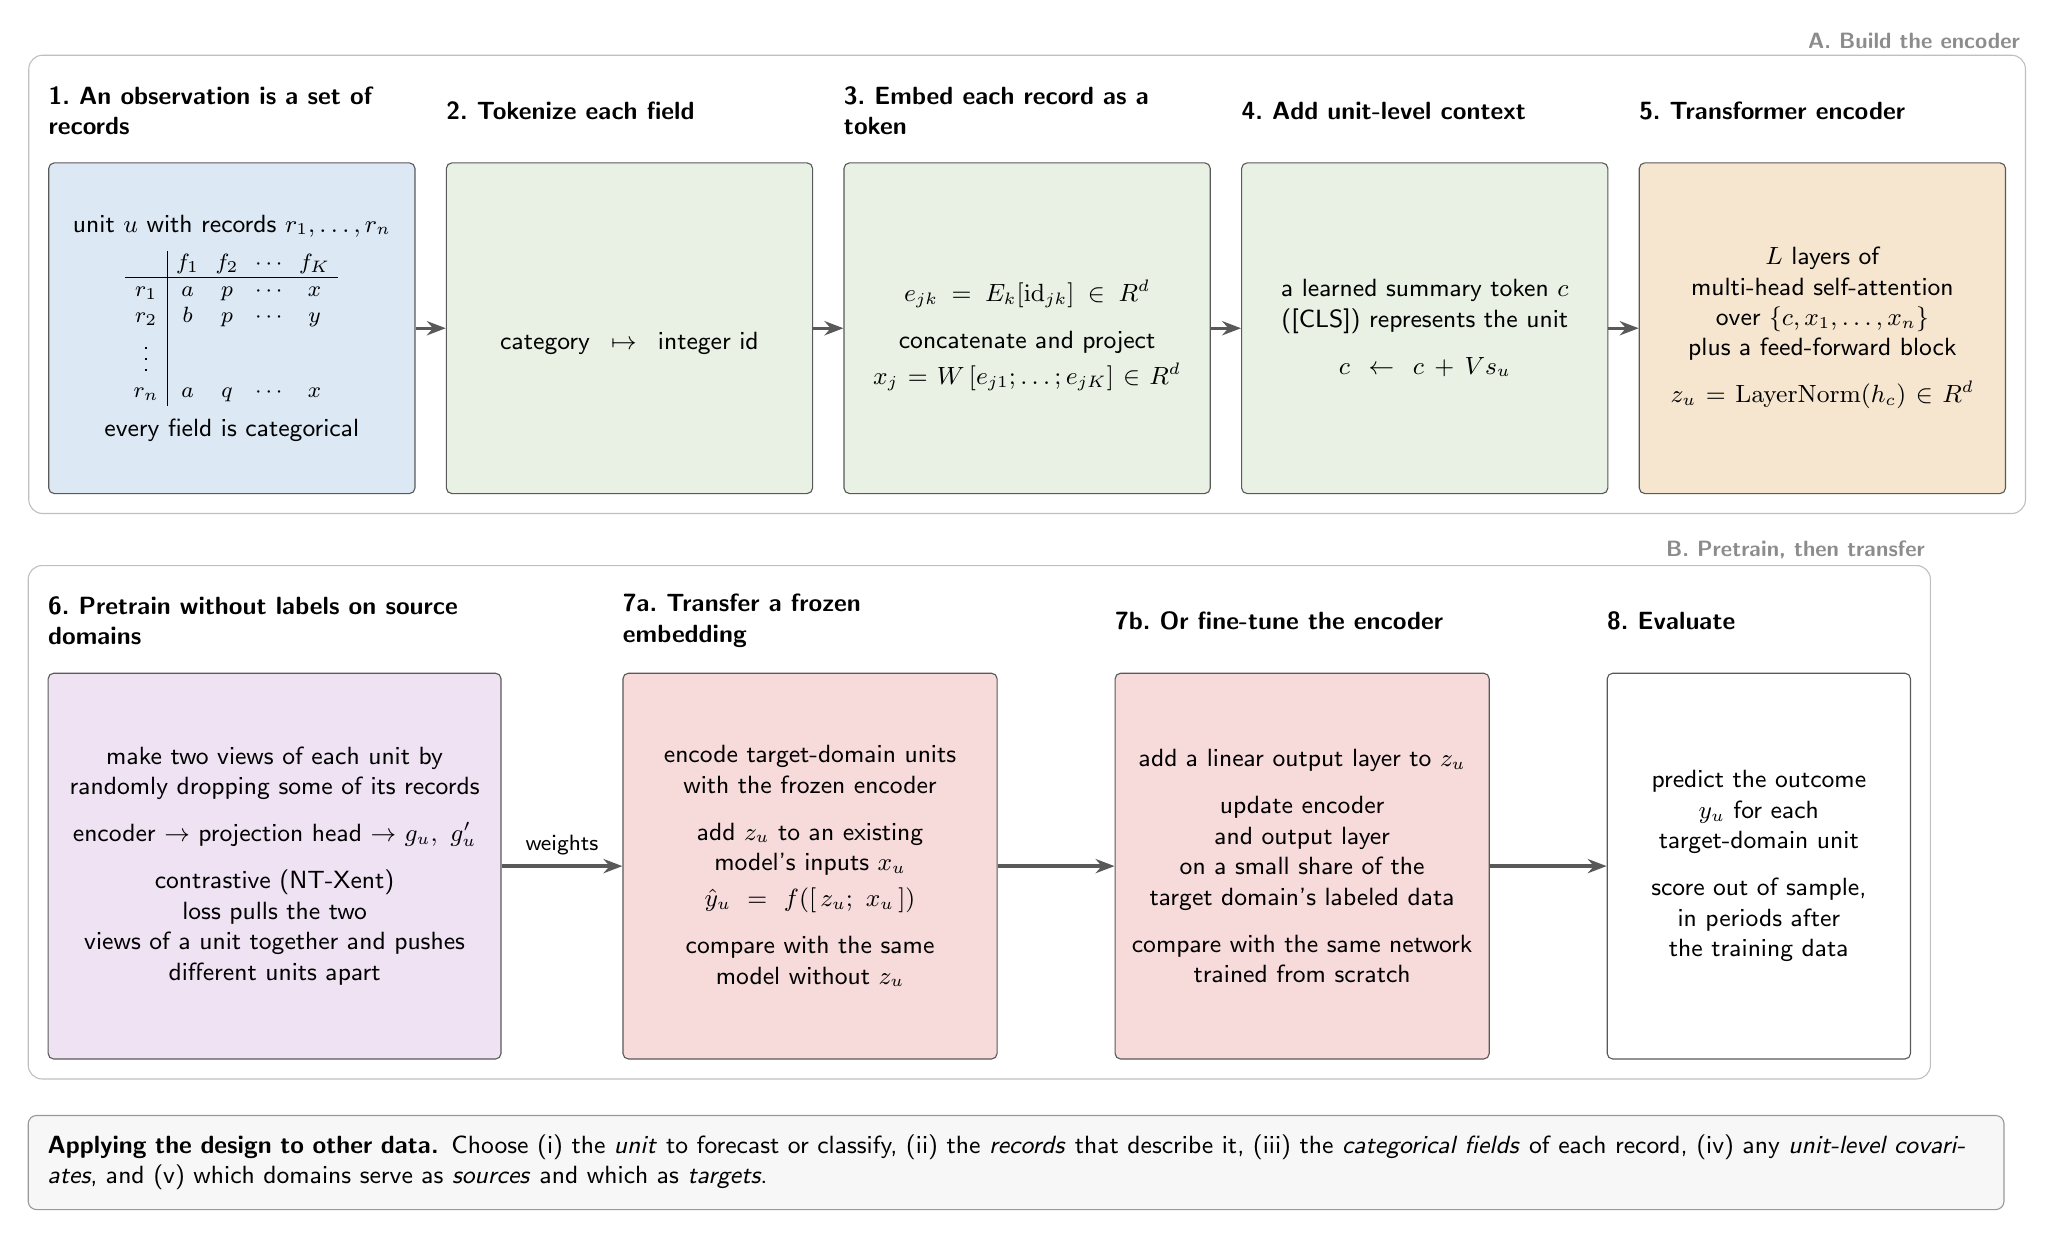
\begin{tikzpicture}[
  font=\sffamily\small,
  >={Stealth[length=2.4mm]},
  hd/.style={font=\sffamily\bfseries\small, text width=4.5cm, align=left, anchor=north west, inner sep=0pt, minimum height=0.9cm,
             execute at begin node={\hyphenpenalty=10000\exhyphenpenalty=10000}},
  bx/.style={draw=black!65, rounded corners=2pt, fill=#1, text width=4.3cm, align=center,
             inner sep=5pt, anchor=north west, minimum height=4.2cm,
             execute at begin node={\hyphenpenalty=10000\exhyphenpenalty=10000}},
  bx/.default=white,
  nt/.style={font=\sffamily\footnotesize\itshape, text=black!55, text width=4.5cm, align=left,
             execute at begin node={\hyphenpenalty=10000\exhyphenpenalty=10000},
             anchor=north west, inner sep=0pt},
  arr/.style={->, very thick, draw=black!65},
  panel/.style={draw=black!25, rounded corners=5pt, inner sep=7pt},
  ptag/.style={font=\sffamily\bfseries\footnotesize, text=black!45, anchor=south east, inner sep=2pt}
]
\definecolor{cIn}{HTML}{DCE9F5}
\definecolor{cTok}{HTML}{E8F1E4}
\definecolor{cEnc}{HTML}{F6E6CF}
\definecolor{cPre}{HTML}{EFE3F3}
\definecolor{cTr}{HTML}{F7DADA}

% ======================= Panel A: build the encoder =======================
\def\xA{0}\def\xB{5.05}\def\xC{10.1}\def\xD{15.15}\def\xE{20.2}

\node[hd] (h1) at (\xA,0) {1.\ An observation is a set of records};
\node[bx=cIn, below=2mm of h1.south west, anchor=north west] (b1)
  {unit $u$ with records $r_1,\dots,r_n$\\[4pt]
   {\footnotesize\setlength{\tabcolsep}{3pt}%
   \begin{tabular}{c|cccc}
            & $f_1$ & $f_2$ & $\cdots$ & $f_K$\\\hline
   $r_1$    & $a$     & $p$     & $\cdots$ & $x$\\
   $r_2$    & $b$     & $p$     & $\cdots$ & $y$\\
   $\vdots$ &         &         &          &    \\
   $r_n$    & $a$     & $q$     & $\cdots$ & $x$
   \end{tabular}}\\[4pt]
   every field is categorical};

\node[hd] (h2) at (\xB,0) {2.\ Tokenize each field};
\node[bx=cTok, below=2mm of h2.south west, anchor=north west] (b2)
  {\\[6pt]
   category $\;\mapsto\;$ integer id\\[6pt]
   };

\node[hd] (h3) at (\xC,0) {3.\ Embed each record as a token};
\node[bx=cTok, below=2mm of h3.south west, anchor=north west] (b3)
  {\\[2pt]
   $e_{jk} = E_k[\mathrm{id}_{jk}] \in \mathbb{R}^{d}$\\[6pt]
   concatenate and project\\[2pt]
   $x_j = W\,[e_{j1};\ldots;e_{jK}] \in \mathbb{R}^{d}$\\[6pt]
   };

\node[hd] (h4) at (\xD,0) {4.\ Add unit-level context};
\node[bx=cTok, below=2mm of h4.south west, anchor=north west] (b4)
  {a learned summary token $c$\\ ([CLS]) represents the unit\\[6pt]
   $c \leftarrow c + V s_u$\\[6pt]
   };

\node[hd] (h5) at (\xE,0) {5.\ Transformer encoder};
\node[bx=cEnc, below=2mm of h5.south west, anchor=north west] (b5)
  {$L$ layers of\\ multi-head self-attention\\ over $\{c, x_1, \ldots, x_n\}$\\ plus a feed-forward block\\[6pt]
   $z_u = \mathrm{LayerNorm}(h_{c}) \in \mathbb{R}^{d}$};

\draw[arr] (b1.east) -- (b2.west);
\draw[arr] (b2.east) -- (b3.west);
\draw[arr] (b3.east) -- (b4.west);
\draw[arr] (b4.east) -- (b5.west);

\begin{scope}[on background layer]
  \node[panel, fit={(h1) (b1) (b2) (b3) (b4) (b5) (h5)}] (pA) {};
\end{scope}
\node[ptag] at (pA.north east) {A.\ Build the encoder};

% ======================= Panel B: pretrain, then transfer =======================
\coordinate (rowB) at ($(pA.south west)+(7pt,-0.9)$);

\node[hd, text width=5.6cm] (h6) at (rowB) {6.\ Pretrain without labels on source domains};
\node[bx=cPre, text width=5.4cm, minimum height=4.9cm, below=2mm of h6.south west, anchor=north west] (b6)
  {make two views of each unit by\\ randomly dropping some of its records\\[6pt]
   encoder $\rightarrow$ projection head $\rightarrow$ $g_u,\ g'_u$\\[6pt]
   contrastive (NT-Xent) loss pulls the two\\ views of a unit together and pushes\\ different units apart};

\node[hd, text width=4.6cm] (h7) at ($(rowB)+(7.3,0)$) {7a.\ Transfer a frozen embedding};
\node[bx=cTr, text width=4.4cm, minimum height=4.9cm, below=2mm of h7.south west, anchor=north west] (b7)
  {encode target-domain units\\ with the frozen encoder\\[6pt]
   add $z_u$ to an existing\\ model's inputs $x_u$\\[2pt]
   $\hat{y}_u = f([\,z_u;\ x_u\,])$\\[6pt]
   compare with the same\\ model without $z_u$};

\node[hd, text width=4.6cm] (h8) at ($(rowB)+(13.55,0)$) {7b.\ Or fine-tune the encoder};
\node[bx=cTr, text width=4.4cm, minimum height=4.9cm, below=2mm of h8.south west, anchor=north west] (b8)
  {add a linear output layer to $z_u$\\[6pt]
   update encoder and output layer\\ on a small share of the\\ target domain's labeled data\\[6pt]
   compare with the same network\\ trained from scratch};

\node[hd, text width=3.6cm] (h9) at ($(rowB)+(19.8,0)$) {8.\ Evaluate};
\node[bx, text width=3.5cm, minimum height=4.9cm, below=2mm of h9.south west, anchor=north west] (b9)
  {predict the outcome\\ $y_u$ for each\\ target-domain unit\\[6pt]
   score out of sample,\\ in periods after\\ the training data};

\draw[arr] (b6.east) -- node[above, font=\sffamily\footnotesize]{weights} (b7.west);
\draw[arr] (b7.east) -- (b8.west);
\draw[arr] (b8.east) -- (b9.west);

\begin{scope}[on background layer]
  \node[panel, fit={(h6) (b6) (b7) (b8) (h9) (b9)}] (pB) {};
\end{scope}
\node[ptag] at (pB.north east) {B.\ Pretrain, then transfer};

% ======================= Reuse box =======================
\node[draw=black!40, fill=black!3, rounded corners=3pt, anchor=north west, inner sep=7pt,
      text width=24.6cm, align=left, font=\sffamily\small]
  (reuse) at ($(pB.south west)+(0,-0.45)$)
  {\textbf{Applying the design to other data.} Choose (i) the \emph{unit} to forecast or classify, (ii) the \emph{records} that describe it,
   (iii) the \emph{categorical fields} of each record, (iv) any \emph{unit-level covariates}, and (v) which domains serve as \emph{sources} and which as \emph{targets}.};%\\[4pt]
   %{\footnotesize\textit{Roll-call voting}: unit = legislator-session; records = votes; fields = bill topic, vote cast, sponsor party, committee.
   %\quad \textit{Alliances}: unit = state dyad-year; records = treaty provisions; fields = obligation type, scope, partner region.
   %\quad \textit{Protest}: unit = user-week; records = online actions; fields = action type, target, tie type.}};
\end{tikzpicture}%
}
\caption{Building a transformer encoder for structured data. Panel A turns an observation made of many categorical records into a single learned vector. Panel B pretrains the encoder without labels on source domains, then transfers it to a target domain either as a frozen embedding or by fine-tuning. The projection head is a learned mapping used for the pretraining loss. Transfer uses the encoder embedding. The bottom box lists the five decisions needed to apply the design to other political science data.}
\label{fig:architecture}
\end{figure}

\usetikzlibrary{positioning, arrows.meta, fit, backgrounds, calc}
\begin{figure}[t]
\centering
\resizebox{\textwidth}{!}{%
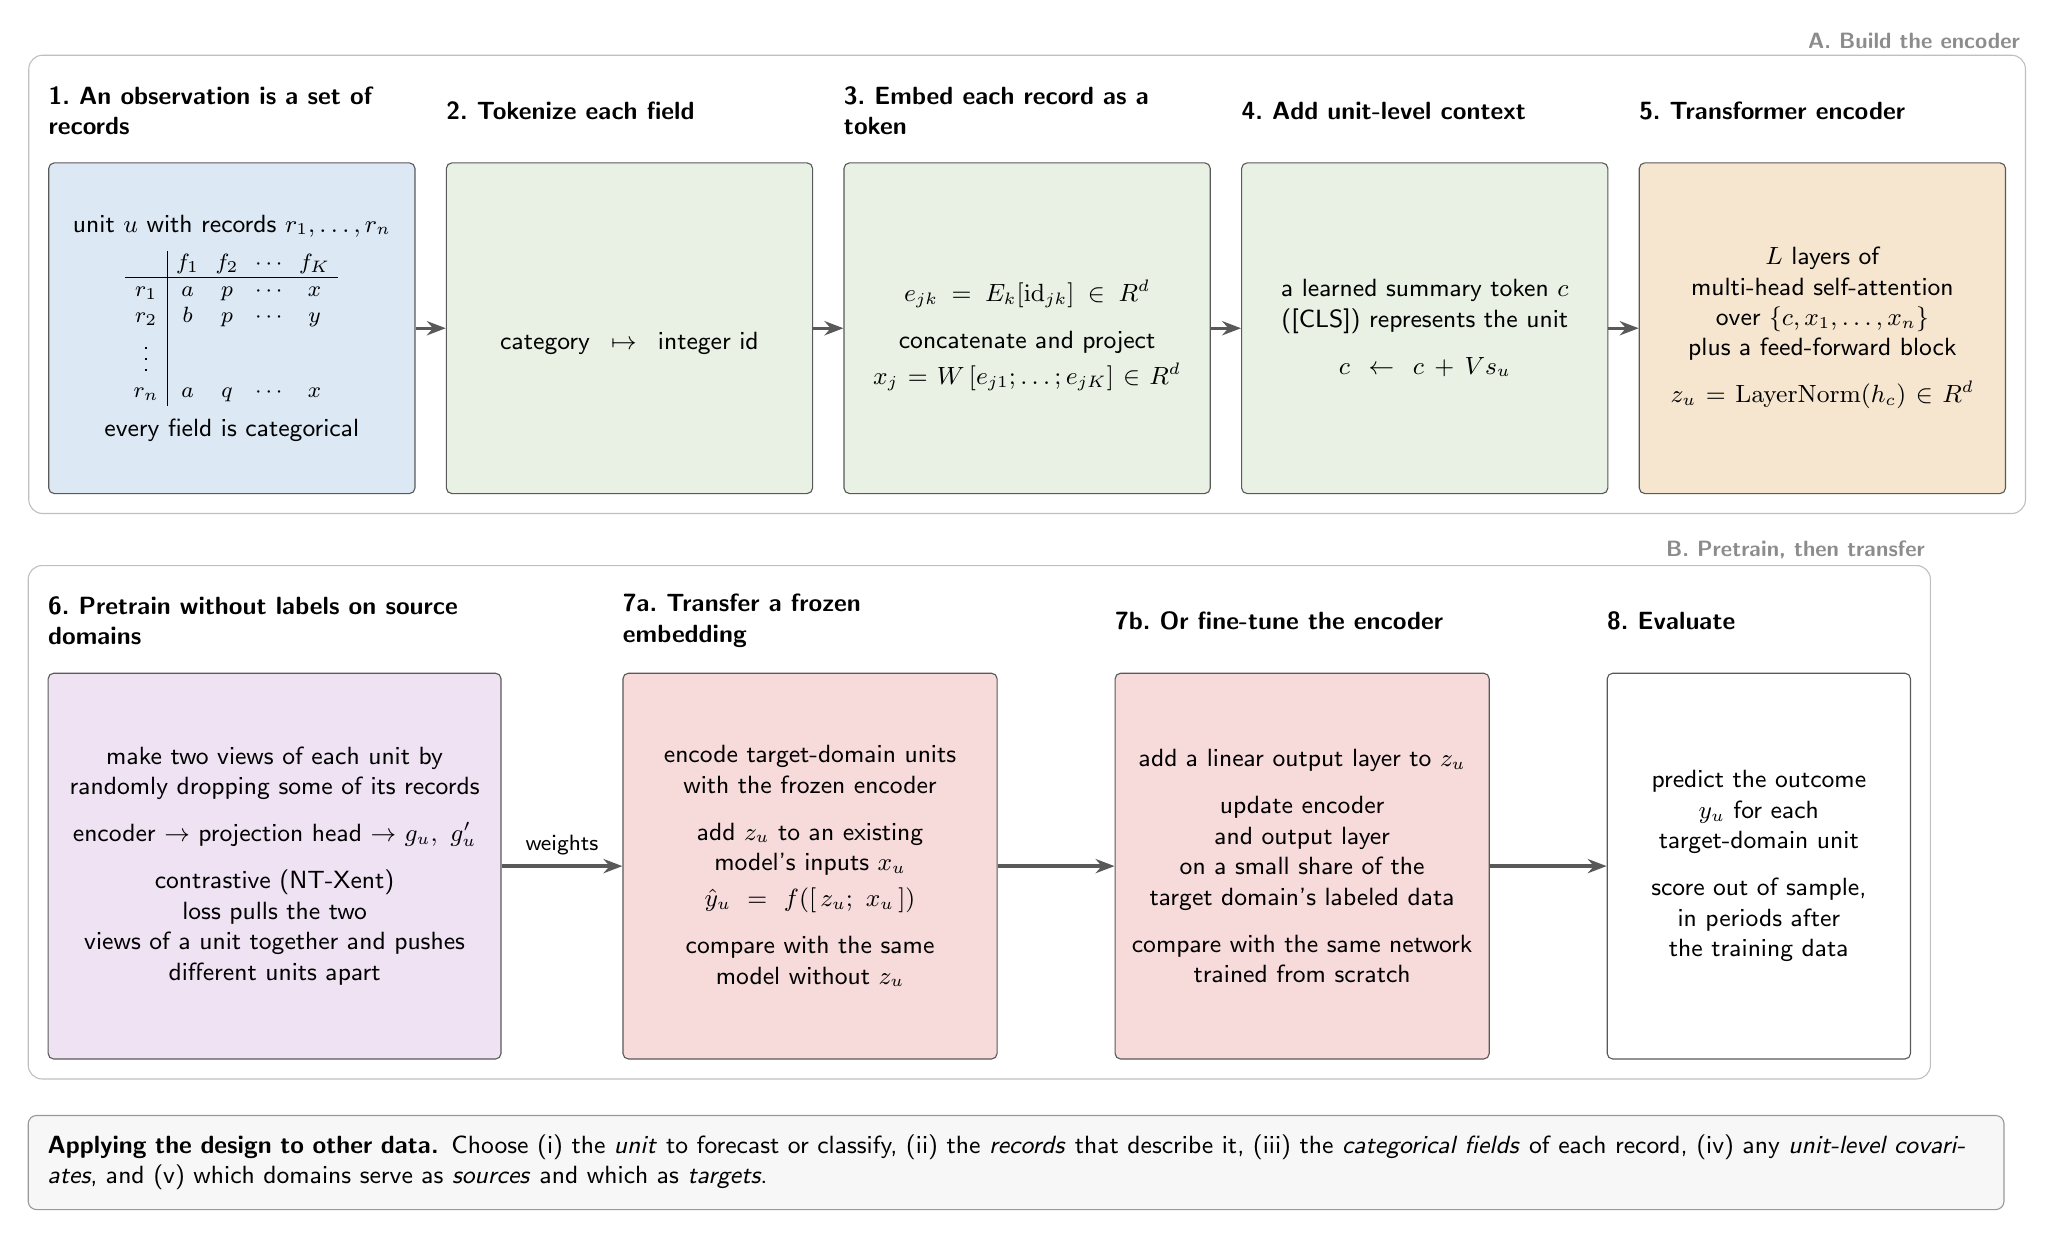
\begin{tikzpicture}[
  font=\sffamily\small,
  >={Stealth[length=2.4mm]},
  hd/.style={font=\sffamily\bfseries\small, text width=4.5cm, align=left, anchor=north west, inner sep=0pt, minimum height=0.9cm,
             execute at begin node={\hyphenpenalty=10000\exhyphenpenalty=10000}},
  bx/.style={draw=black!65, rounded corners=2pt, fill=#1, text width=4.3cm, align=center,
             inner sep=5pt, anchor=north west, minimum height=4.2cm,
             execute at begin node={\hyphenpenalty=10000\exhyphenpenalty=10000}},
  bx/.default=white,
  nt/.style={font=\sffamily\footnotesize\itshape, text=black!55, text width=4.5cm, align=left,
             execute at begin node={\hyphenpenalty=10000\exhyphenpenalty=10000},
             anchor=north west, inner sep=0pt},
  arr/.style={->, very thick, draw=black!65},
  panel/.style={draw=black!25, rounded corners=5pt, inner sep=7pt},
  ptag/.style={font=\sffamily\bfseries\footnotesize, text=black!45, anchor=south east, inner sep=2pt}
]
\definecolor{cIn}{HTML}{DCE9F5}
\definecolor{cTok}{HTML}{E8F1E4}
\definecolor{cEnc}{HTML}{F6E6CF}
\definecolor{cPre}{HTML}{EFE3F3}
\definecolor{cTr}{HTML}{F7DADA}

% ======================= Panel A: build the encoder =======================
\def\xA{0}\def\xB{5.05}\def\xC{10.1}\def\xD{15.15}\def\xE{20.2}

\node[hd] (h1) at (\xA,0) {1.\ An observation is a set of records};
\node[bx=cIn, below=2mm of h1.south west, anchor=north west] (b1)
  {unit $u$ with records $r_1,\dots,r_n$\\[4pt]
   {\footnotesize\setlength{\tabcolsep}{3pt}%
   \begin{tabular}{c|cccc}
            & $f_1$ & $f_2$ & $\cdots$ & $f_K$\\\hline
   $r_1$    & $a$     & $p$     & $\cdots$ & $x$\\
   $r_2$    & $b$     & $p$     & $\cdots$ & $y$\\
   $\vdots$ &         &         &          &    \\
   $r_n$    & $a$     & $q$     & $\cdots$ & $x$
   \end{tabular}}\\[4pt]
   every field is categorical};

\node[hd] (h2) at (\xB,0) {2.\ Tokenize each field};
\node[bx=cTok, below=2mm of h2.south west, anchor=north west] (b2)
  {\\[6pt]
   category $\;\mapsto\;$ integer id\\[6pt]
   };

\node[hd] (h3) at (\xC,0) {3.\ Embed each record as a token};
\node[bx=cTok, below=2mm of h3.south west, anchor=north west] (b3)
  {\\[2pt]
   $e_{jk} = E_k[\mathrm{id}_{jk}] \in \mathbb{R}^{d}$\\[6pt]
   concatenate and project\\[2pt]
   $x_j = W\,[e_{j1};\ldots;e_{jK}] \in \mathbb{R}^{d}$\\[6pt]
   };

\node[hd] (h4) at (\xD,0) {4.\ Add unit-level context};
\node[bx=cTok, below=2mm of h4.south west, anchor=north west] (b4)
  {a learned summary token $c$\\ ([CLS]) represents the unit\\[6pt]
   $c \leftarrow c + V s_u$\\[6pt]
   };

\node[hd] (h5) at (\xE,0) {5.\ Transformer encoder};
\node[bx=cEnc, below=2mm of h5.south west, anchor=north west] (b5)
  {$L$ layers of\\ multi-head self-attention\\ over $\{c, x_1, \ldots, x_n\}$\\ plus a feed-forward block\\[6pt]
   $z_u = \mathrm{LayerNorm}(h_{c}) \in \mathbb{R}^{d}$};

\draw[arr] (b1.east) -- (b2.west);
\draw[arr] (b2.east) -- (b3.west);
\draw[arr] (b3.east) -- (b4.west);
\draw[arr] (b4.east) -- (b5.west);

\begin{scope}[on background layer]
  \node[panel, fit={(h1) (b1) (b2) (b3) (b4) (b5) (h5)}] (pA) {};
\end{scope}
\node[ptag] at (pA.north east) {A.\ Build the encoder};

% ======================= Panel B: pretrain, then transfer =======================
\coordinate (rowB) at ($(pA.south west)+(7pt,-0.9)$);

\node[hd, text width=5.6cm] (h6) at (rowB) {6.\ Pretrain without labels on source domains};
\node[bx=cPre, text width=5.4cm, minimum height=4.9cm, below=2mm of h6.south west, anchor=north west] (b6)
  {make two views of each unit by\\ randomly dropping some of its records\\[6pt]
   encoder $\rightarrow$ projection head $\rightarrow$ $g_u,\ g'_u$\\[6pt]
   contrastive (NT-Xent) loss pulls the two\\ views of a unit together and pushes\\ different units apart};

\node[hd, text width=4.6cm] (h7) at ($(rowB)+(7.3,0)$) {7a.\ Transfer a frozen embedding};
\node[bx=cTr, text width=4.4cm, minimum height=4.9cm, below=2mm of h7.south west, anchor=north west] (b7)
  {encode target-domain units\\ with the frozen encoder\\[6pt]
   add $z_u$ to an existing\\ model's inputs $x_u$\\[2pt]
   $\hat{y}_u = f([\,z_u;\ x_u\,])$\\[6pt]
   compare with the same\\ model without $z_u$};

\node[hd, text width=4.6cm] (h8) at ($(rowB)+(13.55,0)$) {7b.\ Or fine-tune the encoder};
\node[bx=cTr, text width=4.4cm, minimum height=4.9cm, below=2mm of h8.south west, anchor=north west] (b8)
  {add a linear output layer to $z_u$\\[6pt]
   update encoder and output layer\\ on a small share of the\\ target domain's labeled data\\[6pt]
   compare with the same network\\ trained from scratch};

\node[hd, text width=3.6cm] (h9) at ($(rowB)+(19.8,0)$) {8.\ Evaluate};
\node[bx, text width=3.5cm, minimum height=4.9cm, below=2mm of h9.south west, anchor=north west] (b9)
  {predict the outcome\\ $y_u$ for each\\ target-domain unit\\[6pt]
   score out of sample,\\ in periods after\\ the training data};

\draw[arr] (b6.east) -- node[above, font=\sffamily\footnotesize]{weights} (b7.west);
\draw[arr] (b7.east) -- (b8.west);
\draw[arr] (b8.east) -- (b9.west);

\begin{scope}[on background layer]
  \node[panel, fit={(h6) (b6) (b7) (b8) (h9) (b9)}] (pB) {};
\end{scope}
\node[ptag] at (pB.north east) {B.\ Pretrain, then transfer};

% ======================= Reuse box =======================
\node[draw=black!40, fill=black!3, rounded corners=3pt, anchor=north west, inner sep=7pt,
      text width=24.6cm, align=left, font=\sffamily\small]
  (reuse) at ($(pB.south west)+(0,-0.45)$)
  {\textbf{Applying the design to other data.} Choose (i) the \emph{unit} to forecast or classify, (ii) the \emph{records} that describe it,
   (iii) the \emph{categorical fields} of each record, (iv) any \emph{unit-level covariates}, and (v) which domains serve as \emph{sources} and which as \emph{targets}.};%\\[4pt]
   %{\footnotesize\textit{Roll-call voting}: unit = legislator-session; records = votes; fields = bill topic, vote cast, sponsor party, committee.
   %\quad \textit{Alliances}: unit = state dyad-year; records = treaty provisions; fields = obligation type, scope, partner region.
   %\quad \textit{Protest}: unit = user-week; records = online actions; fields = action type, target, tie type.}};
\end{tikzpicture}%
}
\caption{Building a transformer encoder for structured data. Panel A turns an observation made of many categorical records into a single learned vector. Panel B pretrains the encoder without labels on source domains, then transfers it to a target domain either as a frozen embedding or by fine-tuning. The projection head is a learned mapping used for the pretraining loss. Transfer uses the encoder embedding. The bottom box lists the five decisions needed to apply the design to other political science data.}
\label{fig:architecture}
\end{figure}

\usetikzlibrary{positioning, arrows.meta, fit, backgrounds, calc}
\begin{figure}[t]
\centering
\resizebox{\textwidth}{!}{%
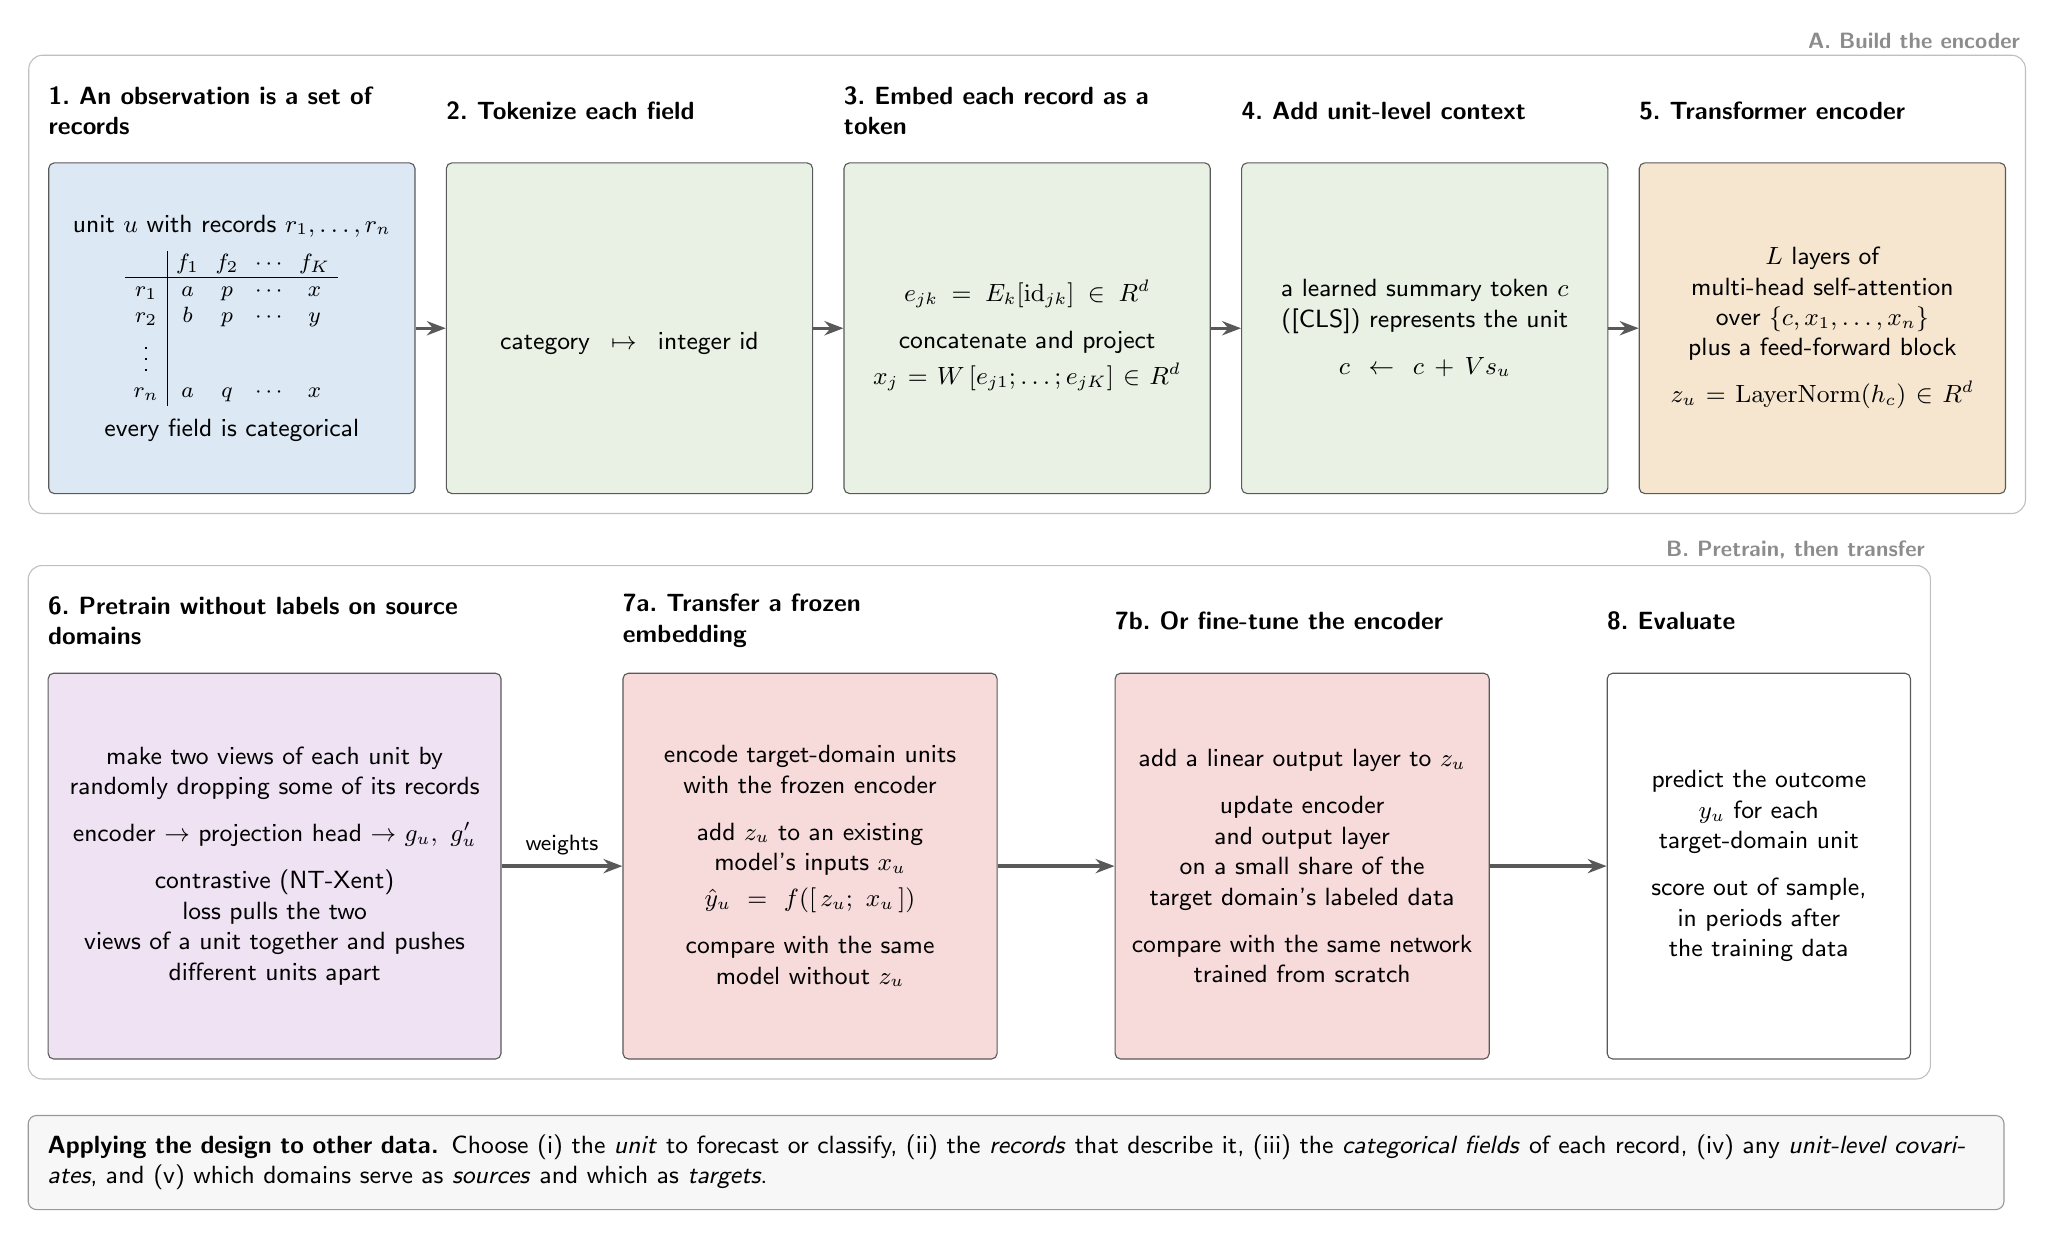
\begin{tikzpicture}[
  font=\sffamily\small,
  >={Stealth[length=2.4mm]},
  hd/.style={font=\sffamily\bfseries\small, text width=4.5cm, align=left, anchor=north west, inner sep=0pt, minimum height=0.9cm,
             execute at begin node={\hyphenpenalty=10000\exhyphenpenalty=10000}},
  bx/.style={draw=black!65, rounded corners=2pt, fill=#1, text width=4.3cm, align=center,
             inner sep=5pt, anchor=north west, minimum height=4.2cm,
             execute at begin node={\hyphenpenalty=10000\exhyphenpenalty=10000}},
  bx/.default=white,
  nt/.style={font=\sffamily\footnotesize\itshape, text=black!55, text width=4.5cm, align=left,
             execute at begin node={\hyphenpenalty=10000\exhyphenpenalty=10000},
             anchor=north west, inner sep=0pt},
  arr/.style={->, very thick, draw=black!65},
  panel/.style={draw=black!25, rounded corners=5pt, inner sep=7pt},
  ptag/.style={font=\sffamily\bfseries\footnotesize, text=black!45, anchor=south east, inner sep=2pt}
]
\definecolor{cIn}{HTML}{DCE9F5}
\definecolor{cTok}{HTML}{E8F1E4}
\definecolor{cEnc}{HTML}{F6E6CF}
\definecolor{cPre}{HTML}{EFE3F3}
\definecolor{cTr}{HTML}{F7DADA}

% ======================= Panel A: build the encoder =======================
\def\xA{0}\def\xB{5.05}\def\xC{10.1}\def\xD{15.15}\def\xE{20.2}

\node[hd] (h1) at (\xA,0) {1.\ An observation is a set of records};
\node[bx=cIn, below=2mm of h1.south west, anchor=north west] (b1)
  {unit $u$ with records $r_1,\dots,r_n$\\[4pt]
   {\footnotesize\setlength{\tabcolsep}{3pt}%
   \begin{tabular}{c|cccc}
            & $f_1$ & $f_2$ & $\cdots$ & $f_K$\\\hline
   $r_1$    & $a$     & $p$     & $\cdots$ & $x$\\
   $r_2$    & $b$     & $p$     & $\cdots$ & $y$\\
   $\vdots$ &         &         &          &    \\
   $r_n$    & $a$     & $q$     & $\cdots$ & $x$
   \end{tabular}}\\[4pt]
   every field is categorical};

\node[hd] (h2) at (\xB,0) {2.\ Tokenize each field};
\node[bx=cTok, below=2mm of h2.south west, anchor=north west] (b2)
  {\\[6pt]
   category $\;\mapsto\;$ integer id\\[6pt]
   };

\node[hd] (h3) at (\xC,0) {3.\ Embed each record as a token};
\node[bx=cTok, below=2mm of h3.south west, anchor=north west] (b3)
  {\\[2pt]
   $e_{jk} = E_k[\mathrm{id}_{jk}] \in \mathbb{R}^{d}$\\[6pt]
   concatenate and project\\[2pt]
   $x_j = W\,[e_{j1};\ldots;e_{jK}] \in \mathbb{R}^{d}$\\[6pt]
   };

\node[hd] (h4) at (\xD,0) {4.\ Add unit-level context};
\node[bx=cTok, below=2mm of h4.south west, anchor=north west] (b4)
  {a learned summary token $c$\\ ([CLS]) represents the unit\\[6pt]
   $c \leftarrow c + V s_u$\\[6pt]
   };

\node[hd] (h5) at (\xE,0) {5.\ Transformer encoder};
\node[bx=cEnc, below=2mm of h5.south west, anchor=north west] (b5)
  {$L$ layers of\\ multi-head self-attention\\ over $\{c, x_1, \ldots, x_n\}$\\ plus a feed-forward block\\[6pt]
   $z_u = \mathrm{LayerNorm}(h_{c}) \in \mathbb{R}^{d}$};

\draw[arr] (b1.east) -- (b2.west);
\draw[arr] (b2.east) -- (b3.west);
\draw[arr] (b3.east) -- (b4.west);
\draw[arr] (b4.east) -- (b5.west);

\begin{scope}[on background layer]
  \node[panel, fit={(h1) (b1) (b2) (b3) (b4) (b5) (h5)}] (pA) {};
\end{scope}
\node[ptag] at (pA.north east) {A.\ Build the encoder};

% ======================= Panel B: pretrain, then transfer =======================
\coordinate (rowB) at ($(pA.south west)+(7pt,-0.9)$);

\node[hd, text width=5.6cm] (h6) at (rowB) {6.\ Pretrain without labels on source domains};
\node[bx=cPre, text width=5.4cm, minimum height=4.9cm, below=2mm of h6.south west, anchor=north west] (b6)
  {make two views of each unit by\\ randomly dropping some of its records\\[6pt]
   encoder $\rightarrow$ projection head $\rightarrow$ $g_u,\ g'_u$\\[6pt]
   contrastive (NT-Xent) loss pulls the two\\ views of a unit together and pushes\\ different units apart};

\node[hd, text width=4.6cm] (h7) at ($(rowB)+(7.3,0)$) {7a.\ Transfer a frozen embedding};
\node[bx=cTr, text width=4.4cm, minimum height=4.9cm, below=2mm of h7.south west, anchor=north west] (b7)
  {encode target-domain units\\ with the frozen encoder\\[6pt]
   add $z_u$ to an existing\\ model's inputs $x_u$\\[2pt]
   $\hat{y}_u = f([\,z_u;\ x_u\,])$\\[6pt]
   compare with the same\\ model without $z_u$};

\node[hd, text width=4.6cm] (h8) at ($(rowB)+(13.55,0)$) {7b.\ Or fine-tune the encoder};
\node[bx=cTr, text width=4.4cm, minimum height=4.9cm, below=2mm of h8.south west, anchor=north west] (b8)
  {add a linear output layer to $z_u$\\[6pt]
   update encoder and output layer\\ on a small share of the\\ target domain's labeled data\\[6pt]
   compare with the same network\\ trained from scratch};

\node[hd, text width=3.6cm] (h9) at ($(rowB)+(19.8,0)$) {8.\ Evaluate};
\node[bx, text width=3.5cm, minimum height=4.9cm, below=2mm of h9.south west, anchor=north west] (b9)
  {predict the outcome\\ $y_u$ for each\\ target-domain unit\\[6pt]
   score out of sample,\\ in periods after\\ the training data};

\draw[arr] (b6.east) -- node[above, font=\sffamily\footnotesize]{weights} (b7.west);
\draw[arr] (b7.east) -- (b8.west);
\draw[arr] (b8.east) -- (b9.west);

\begin{scope}[on background layer]
  \node[panel, fit={(h6) (b6) (b7) (b8) (h9) (b9)}] (pB) {};
\end{scope}
\node[ptag] at (pB.north east) {B.\ Pretrain, then transfer};

% ======================= Reuse box =======================
\node[draw=black!40, fill=black!3, rounded corners=3pt, anchor=north west, inner sep=7pt,
      text width=24.6cm, align=left, font=\sffamily\small]
  (reuse) at ($(pB.south west)+(0,-0.45)$)
  {\textbf{Applying the design to other data.} Choose (i) the \emph{unit} to forecast or classify, (ii) the \emph{records} that describe it,
   (iii) the \emph{categorical fields} of each record, (iv) any \emph{unit-level covariates}, and (v) which domains serve as \emph{sources} and which as \emph{targets}.};%\\[4pt]
   %{\footnotesize\textit{Roll-call voting}: unit = legislator-session; records = votes; fields = bill topic, vote cast, sponsor party, committee.
   %\quad \textit{Alliances}: unit = state dyad-year; records = treaty provisions; fields = obligation type, scope, partner region.
   %\quad \textit{Protest}: unit = user-week; records = online actions; fields = action type, target, tie type.}};
\end{tikzpicture}%
}
\caption{Building a transformer encoder for structured data. Panel A turns an observation made of many categorical records into a single learned vector. Panel B pretrains the encoder without labels on source domains, then transfers it to a target domain either as a frozen embedding or by fine-tuning. The projection head is a learned mapping used for the pretraining loss. Transfer uses the encoder embedding. The bottom box lists the five decisions needed to apply the design to other political science data.}
\label{fig:architecture}
\end{figure}

\usetikzlibrary{positioning, arrows.meta, fit, backgrounds, calc}
\begin{figure}[t]
\centering
\resizebox{\textwidth}{!}{%
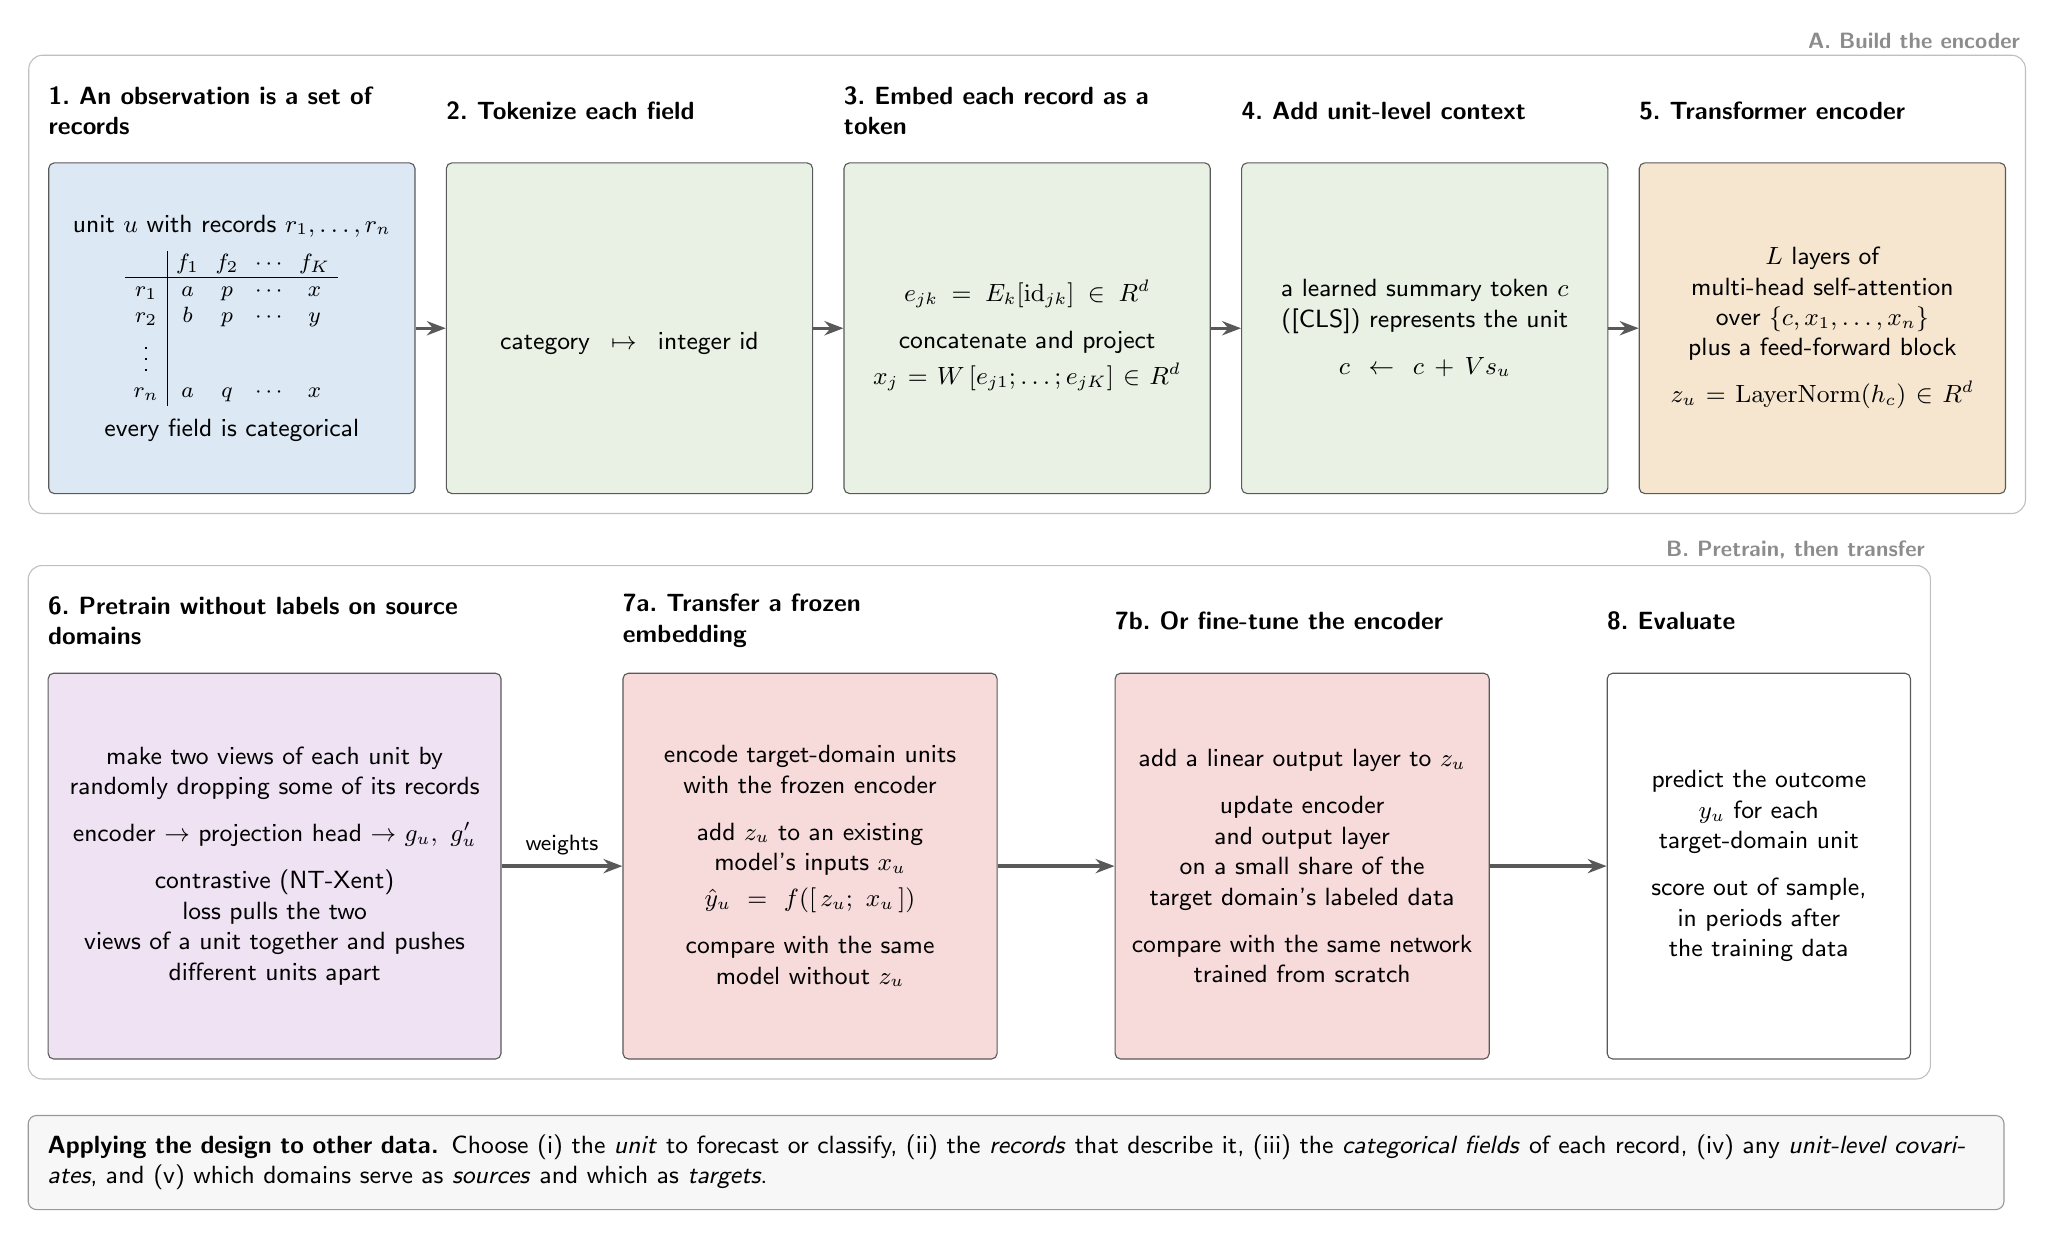
\begin{tikzpicture}[
  font=\sffamily\small,
  >={Stealth[length=2.4mm]},
  hd/.style={font=\sffamily\bfseries\small, text width=4.5cm, align=left, anchor=north west, inner sep=0pt, minimum height=0.9cm,
             execute at begin node={\hyphenpenalty=10000\exhyphenpenalty=10000}},
  bx/.style={draw=black!65, rounded corners=2pt, fill=#1, text width=4.3cm, align=center,
             inner sep=5pt, anchor=north west, minimum height=4.2cm,
             execute at begin node={\hyphenpenalty=10000\exhyphenpenalty=10000}},
  bx/.default=white,
  nt/.style={font=\sffamily\footnotesize\itshape, text=black!55, text width=4.5cm, align=left,
             execute at begin node={\hyphenpenalty=10000\exhyphenpenalty=10000},
             anchor=north west, inner sep=0pt},
  arr/.style={->, very thick, draw=black!65},
  panel/.style={draw=black!25, rounded corners=5pt, inner sep=7pt},
  ptag/.style={font=\sffamily\bfseries\footnotesize, text=black!45, anchor=south east, inner sep=2pt}
]
\definecolor{cIn}{HTML}{DCE9F5}
\definecolor{cTok}{HTML}{E8F1E4}
\definecolor{cEnc}{HTML}{F6E6CF}
\definecolor{cPre}{HTML}{EFE3F3}
\definecolor{cTr}{HTML}{F7DADA}

% ======================= Panel A: build the encoder =======================
\def\xA{0}\def\xB{5.05}\def\xC{10.1}\def\xD{15.15}\def\xE{20.2}

\node[hd] (h1) at (\xA,0) {1.\ An observation is a set of records};
\node[bx=cIn, below=2mm of h1.south west, anchor=north west] (b1)
  {unit $u$ with records $r_1,\dots,r_n$\\[4pt]
   {\footnotesize\setlength{\tabcolsep}{3pt}%
   \begin{tabular}{c|cccc}
            & $f_1$ & $f_2$ & $\cdots$ & $f_K$\\\hline
   $r_1$    & $a$     & $p$     & $\cdots$ & $x$\\
   $r_2$    & $b$     & $p$     & $\cdots$ & $y$\\
   $\vdots$ &         &         &          &    \\
   $r_n$    & $a$     & $q$     & $\cdots$ & $x$
   \end{tabular}}\\[4pt]
   every field is categorical};

\node[hd] (h2) at (\xB,0) {2.\ Tokenize each field};
\node[bx=cTok, below=2mm of h2.south west, anchor=north west] (b2)
  {\\[6pt]
   category $\;\mapsto\;$ integer id\\[6pt]
   };

\node[hd] (h3) at (\xC,0) {3.\ Embed each record as a token};
\node[bx=cTok, below=2mm of h3.south west, anchor=north west] (b3)
  {\\[2pt]
   $e_{jk} = E_k[\mathrm{id}_{jk}] \in \mathbb{R}^{d}$\\[6pt]
   concatenate and project\\[2pt]
   $x_j = W\,[e_{j1};\ldots;e_{jK}] \in \mathbb{R}^{d}$\\[6pt]
   };

\node[hd] (h4) at (\xD,0) {4.\ Add unit-level context};
\node[bx=cTok, below=2mm of h4.south west, anchor=north west] (b4)
  {a learned summary token $c$\\ ([CLS]) represents the unit\\[6pt]
   $c \leftarrow c + V s_u$\\[6pt]
   };

\node[hd] (h5) at (\xE,0) {5.\ Transformer encoder};
\node[bx=cEnc, below=2mm of h5.south west, anchor=north west] (b5)
  {$L$ layers of\\ multi-head self-attention\\ over $\{c, x_1, \ldots, x_n\}$\\ plus a feed-forward block\\[6pt]
   $z_u = \mathrm{LayerNorm}(h_{c}) \in \mathbb{R}^{d}$};

\draw[arr] (b1.east) -- (b2.west);
\draw[arr] (b2.east) -- (b3.west);
\draw[arr] (b3.east) -- (b4.west);
\draw[arr] (b4.east) -- (b5.west);

\begin{scope}[on background layer]
  \node[panel, fit={(h1) (b1) (b2) (b3) (b4) (b5) (h5)}] (pA) {};
\end{scope}
\node[ptag] at (pA.north east) {A.\ Build the encoder};

% ======================= Panel B: pretrain, then transfer =======================
\coordinate (rowB) at ($(pA.south west)+(7pt,-0.9)$);

\node[hd, text width=5.6cm] (h6) at (rowB) {6.\ Pretrain without labels on source domains};
\node[bx=cPre, text width=5.4cm, minimum height=4.9cm, below=2mm of h6.south west, anchor=north west] (b6)
  {make two views of each unit by\\ randomly dropping some of its records\\[6pt]
   encoder $\rightarrow$ projection head $\rightarrow$ $g_u,\ g'_u$\\[6pt]
   contrastive (NT-Xent) loss pulls the two\\ views of a unit together and pushes\\ different units apart};

\node[hd, text width=4.6cm] (h7) at ($(rowB)+(7.3,0)$) {7a.\ Transfer a frozen embedding};
\node[bx=cTr, text width=4.4cm, minimum height=4.9cm, below=2mm of h7.south west, anchor=north west] (b7)
  {encode target-domain units\\ with the frozen encoder\\[6pt]
   add $z_u$ to an existing\\ model's inputs $x_u$\\[2pt]
   $\hat{y}_u = f([\,z_u;\ x_u\,])$\\[6pt]
   compare with the same\\ model without $z_u$};

\node[hd, text width=4.6cm] (h8) at ($(rowB)+(13.55,0)$) {7b.\ Or fine-tune the encoder};
\node[bx=cTr, text width=4.4cm, minimum height=4.9cm, below=2mm of h8.south west, anchor=north west] (b8)
  {add a linear output layer to $z_u$\\[6pt]
   update encoder and output layer\\ on a small share of the\\ target domain's labeled data\\[6pt]
   compare with the same network\\ trained from scratch};

\node[hd, text width=3.6cm] (h9) at ($(rowB)+(19.8,0)$) {8.\ Evaluate};
\node[bx, text width=3.5cm, minimum height=4.9cm, below=2mm of h9.south west, anchor=north west] (b9)
  {predict the outcome\\ $y_u$ for each\\ target-domain unit\\[6pt]
   score out of sample,\\ in periods after\\ the training data};

\draw[arr] (b6.east) -- node[above, font=\sffamily\footnotesize]{weights} (b7.west);
\draw[arr] (b7.east) -- (b8.west);
\draw[arr] (b8.east) -- (b9.west);

\begin{scope}[on background layer]
  \node[panel, fit={(h6) (b6) (b7) (b8) (h9) (b9)}] (pB) {};
\end{scope}
\node[ptag] at (pB.north east) {B.\ Pretrain, then transfer};

% ======================= Reuse box =======================
\node[draw=black!40, fill=black!3, rounded corners=3pt, anchor=north west, inner sep=7pt,
      text width=24.6cm, align=left, font=\sffamily\small]
  (reuse) at ($(pB.south west)+(0,-0.45)$)
  {\textbf{Applying the design to other data.} Choose (i) the \emph{unit} to forecast or classify, (ii) the \emph{records} that describe it,
   (iii) the \emph{categorical fields} of each record, (iv) any \emph{unit-level covariates}, and (v) which domains serve as \emph{sources} and which as \emph{targets}.};%\\[4pt]
   %{\footnotesize\textit{Roll-call voting}: unit = legislator-session; records = votes; fields = bill topic, vote cast, sponsor party, committee.
   %\quad \textit{Alliances}: unit = state dyad-year; records = treaty provisions; fields = obligation type, scope, partner region.
   %\quad \textit{Protest}: unit = user-week; records = online actions; fields = action type, target, tie type.}};
\end{tikzpicture}%
}
\caption{Building a transformer encoder for structured data. Panel A turns an observation made of many categorical records into a single learned vector. Panel B pretrains the encoder without labels on source domains, then transfers it to a target domain either as a frozen embedding or by fine-tuning. The projection head is a learned mapping used for the pretraining loss. Transfer uses the encoder embedding. The bottom box lists the five decisions needed to apply the design to other political science data.}
\label{fig:architecture}
\end{figure}
